%!TEX root = ../template.tex
%%%%%%%%%%%%%%%%%%%%%%%%%%%%%%%%%%%%%%%%%%%%%%%%%%%%%%%%%%%%%%%%%%%%
%% chapter3.tex
%% NOVA thesis document file
%%
%% Chapter with a short latex tutorial and examples
%%%%%%%%%%%%%%%%%%%%%%%%%%%%%%%%%%%%%%%%%%%%%%%%%%%%%%%%%%%%%%%%%%%%

\typeout{NT FILE chapter3.tex}%


\chapter{Materials and Methods}
\label{cha:materialsandmethods}


\textit{The following section describes the methodologies and workflow of the benchmarking study. 
It begins by describing the input data used, both transcriptomic data and prior knowledge data. 
In addition, it details the implementation of the selected algorithms and their execution. 
Finally, the metrics used to evaluate their performance are described.}

\section{Benchmarking architecture setup} % (fold)
\label{sec:benchmarkingarchitecturesetup}

Several tools and algorithms are available for most research tasks in computational biology, and new algorithms and tools are published every week. 
At the same time, finding the right computational tool for a given research question is essential.
Systematic benchmarking of tools is a time- and resource-consuming endeavor, while a lack of benchmarking carries several potential risks.
Researchers usually carry out published benchmarking to demonstrate that their tool performs better than others. 
\gls{ABC} is a consortium created in 2021 to help members reduce R\&D risks, saving time and resources by distributing the effort of benchmarking computational biology algorithms. 
\gls{ABC} maintains the same workflow regardless of the case study. 
It consists of three main steps: (1) Voting, (2) Curation, and (3) Coding. 
The consortium members suggest and vote on the use case (1). 
Once the use case is determined, the curation phase begins, where Clarivate collects the most appropriate datasets and algorithms according to the voted use case (2). 
Again, the members vote on the final selection of datasets and algorithms (1). 
Finally, the last phases - implementation, execution, and reporting - are conducted by Clarivate (3). 
The project description will fall within the third phase of the workflow, specifically concerning the algorithm's implementation and execution, where I actively participated since all the data was already collected and voted on when I started the project.
A visual representation of the study workflow is provided~\ref{fig:fig3.1.ABCworkflow} and will be explained in detail in the following sections.
The implementation of \gls{ABC} causal regulation use case was carried out by Dr. Alexandr Ishkin and me.
The entire workflow was conducted in \gls{R} Statistical Software (v4.4.1)~\cite{RN159}, and run on a server with an AMD EPYC 7R13 processor featuring 64 logical CPUs and 246 GB of RAM.

\begin{figure}[htbp]
    \centering
    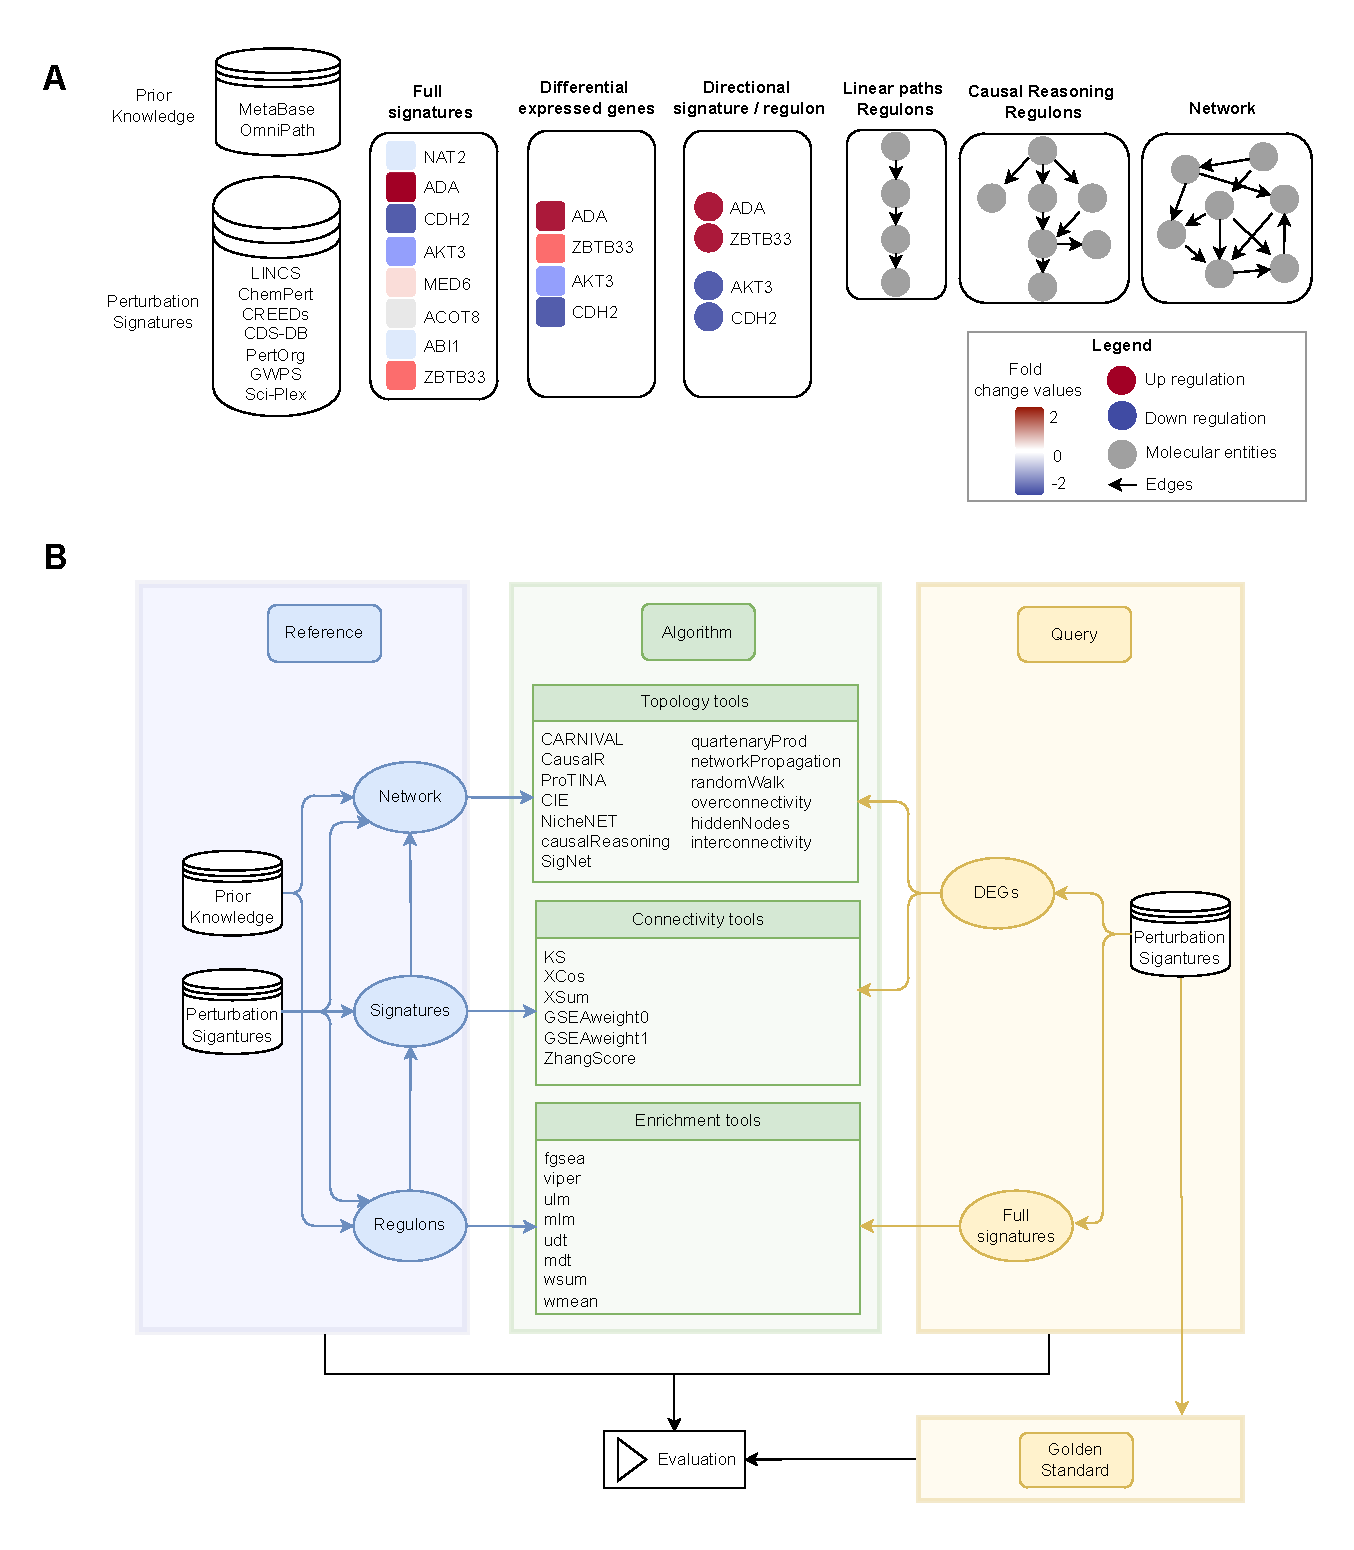
\includegraphics[height=6in]{fig3.1.ABCworkflow}
    \caption[Schematic of the study architecture.]{Schematic of the study architecture. A. Perturbation signatures collected from seven public sources are used in the benchmarking framework either as reference, query, and gold standard (known targets) datasets. Prior knowledge networks, used as reference, were derived from two sources: OmniPath (public) and MetaBase (commercial). From OmniPath, a global network, and regulons were used as references. From MetaBase, it was also used a full network, regulons, and linear pathways. B. Three classes of computational methods were evaluated: topology-based, connectivity-based, and enrichment-based, comprising a total of 27 algorithms. Depending on the method, input data may consist of a global interactome (network), curated signaling pathways, or perturbation signatures (typically directional gene sets or full transcriptomic profiles, which can be reduced to gene sets if needed). These input types are often interrelated, and the arrows in the diagram indicate the required data transformations specific to each algorithm. The output of each method is systematically compared to the gold standard targets for evaluation.}
    \label{fig:fig3.1.ABCworkflow}
\end{figure}

\section{Data Description} % (fold)
\label{sec:datadescription}

As represented in Figure~\ref{fig:fig3.1.ABCworkflow}, each algorithm should receive two types of inputs: query and reference dataset. The query dataset refers to the data derived from perturbed signatures (Full profiles or \gls{DEGs} lists). The reference dataset can be derived either from perturbed signatures (Full profile, \gls{DEGs}, or directional/regulons) or from prior knowledge (Networks or pathways/gene sets). The databases and datasets used as perturbed signatures and as prior knowledge are described below.

\subsection{Gene expression data: Perturbation signatures}
\label{sub:geneexpressiondataperturbationsignatures}

Currently, there are several publicly available perturbation-driven gene expression datasets. This study comprehends transcriptomic datasets from seven different public sources, summarized in Table~\ref{tab:tabel3}. Chemical and genetic perturbagens were included, analyzed by bulk microarray, bulk \gls{RNA-seq}, and \gls{scRNA-seq} assays. Each dataset contains more than hundreds of perturbation signatures. For each collection, the perturbagen type, the total number of unique perturbagens profiled, and the subset for which a gold standard target annotation is available were recorded. The gold standard is necessary for the evaluation and it consists of a set of known targets (drug-protein interactions or genes deliberately perturbed), used to assess the ability of the algorithms to recover true upstream regulators from observed expression changes. 
The \gls{LINCS} expands upon the original \gls{CMap} by leveraging the cost-effective L1000 platform, which directly measures 978 landmark transcripts and imputes the remaining transcriptome to reconstruct genome-wide expression profiles. \gls{LINCS} comprises several distinct collections of perturbations in human cell lines: over 30,000 unique small-molecule treatments, \gls{CRISPR} knockouts targeting 5,156 genes, c\gls{DNA} \gls{OE} of 3,780 genes, and shRNA knockdowns of 4,854 genes. The level 5 data were retrieved from the CLUE platform (available at \href{https://clue.io/data/CMap2020#LINCS2020}{CLUE}). This level already contains the differential expression signatures with z-scores aggregated across biological replicates without p-values.
Since each perturbagen usually appears under multiple conditions (different doses, time points, and cell lines), these were condensed into a single consensus signature per perturbagen by extracting every available gene's z-score and then using the median value across signatures.
For the gold standard, directional effects were assigned as follows: for chemical perturbations \gls{CDDI} annotations were used to identify molecular targets inhibited by specific compounds; for \gls{CRISPR} and \gls{shRNA} datasets, the target genes were assigned with inhibition effect, and for \gls{OE}, each target was assigned with activation effect.

ChemPert is a manually curated compendium of 82,256 gene expression signatures derived from non-cancer cell compound perturbation experiments. Most signatures originate from bulk expression studies in various cell lines, and each is represented as a list of \gls{DEGs} indicating only up- or down-regulation (no fold-change values or p-values). From the total number of signatures, only 2,587 have distinct compounds. A set of consensus \gls{DEGs} lists were derived to reduce redundancy and runtime. For each compound, only genes appearing as \gls{DEGs} in at least two signatures and with the same regulation direction were kept. As well as only signatures with at least 50 consensus \gls{DEGs}. This resulted in 1,304 signatures which was the dataset used instead of the original ChemPert.

\gls{CDS-DB} contains 78 cancer patient-derived, paired pre- and post-treatment transcriptomic datasets, all with associated metadata such as drug dosages, sampling times, and locations. 181 study-level gene perturbation signatures (85 therapeutic regimens across 39 cancer subtypes) were extracted. The perturbagen consists of drugs, and the expression is measured by microarray or \gls{RNA-seq} (including fold change and p-values). 

The sci-Plex dataset is based on a single-cell transcriptomics method that uses nuclear hashing. Sci-Plex dataset profiled three cancer cell lines treated with 188 small-molecule compounds. The data contains full transcriptomic signatures with around 11,000 genes each, containing dose-response effect estimates and associated p-values. Only signatures linked to compounds with known \gls{CDDI} targets were kept. For each of the 135 perturbagen with a target, the gene expression responses were measured across 3 cell lines, resulting in 405 signatures. 

\gls{CREEDS} is a crowd-sourced, manually curated collection of perturbation signatures from \gls{GEO}. Includes both small-molecule and genetic perturbations in mouse and human with the expression from different bulk gene expression platforms. These signatures are represented as \gls{DEGs} lists indicating the regulation direction without fold change values. Only perturbations with \gls{CDDI} target annotations were retained, and all mouse data were mapped to human orthologs, using the metabaser package.

PertOrg is a curated collection of \textit{in vivo} genetic perturbation (such as knockdown, knockout, and overexpression) signatures across 8 model organisms. Only mouse signatures with more than 5,000 genes were kept and mapped to human orthologs. For the gold standard, perturbation effects were considered as activation in the case  of knock-in, overexpression and activation, and inhibition for all the remaining ones. Since PertOrg originally contained 7,398 signatures but only 2,321 distinct target genes, a filtering criteria was applied. Each signature should have at least 50 \gls{DEGs}, and the target gene's fold change should be ranked in the top 5\% by absolute value among all measured genes within that signature. Then, the selected signature was the one with the highest number of \gls{DEGs} per target and perturbation type combination. This resulted in 951 signatures used as PertOrg dataset.

The \gls{GWPS} dataset represents a large-scale effort for single-cell \gls{CRISPR}i profiling across more than 2.5 million human cells. It targets 9,866 genes and was generated using the 10x Genomics platform. The dataset includes 1,946 perturbation signatures corresponding to gene knockdowns. Each signature consists of full transcriptomic profiles by z-scores without p-values. Although the \gls{DEGs} per signature were also provided by the authors, only the full signatures were used in the analysis.

\begin{table}[]
\centering
\caption[Summary of gene expression datasets used in this study.]{Summary of gene expression datasets used in this study. Each dataset includes transcriptomic signatures derived from chemical or genetic perturbations. The Perturbagen column specifies the type of compound or gene perturbation applied, while the Type column labels it as either chemical or genetic. The Number of perturbagens refers to the unique compounds or genes perturbed in the dataset. The Signatures with the gold standard column indicate how many signatures have associated targets that can be used for benchmarking. The Signature type describes the format and content of the signature, such as full profiles or \gls{DEGs} lists.}
\label{tab:tabel3}
\resizebox{\columnwidth}{!}{%
\begin{tabular}{lllllll}
\hline
\textbf{Data set} &
  \textbf{Perturbagen} &
  \textbf{Type} &
  \textbf{\begin{tabular}[c]{@{}l@{}}Number of \\ perturbagens\end{tabular}} &
  \textbf{\begin{tabular}[c]{@{}l@{}}Signatures with \\ gold standard\end{tabular}} &
  \textbf{\begin{tabular}[c]{@{}l@{}}Signature \\ type\end{tabular}} &
  \textbf{Ref.} \\ \hline
\begin{tabular}[c]{@{}l@{}}\gls{LINCS} \\ compounds\end{tabular} &
  Compound (small molecules) &
  Chemical &
  33,627 &
  3,540 &
  Full &
  \cite{RN30} \\
ChemPert &
  \begin{tabular}[c]{@{}l@{}}Compound (small molecules, \\ ligands, drugs)\end{tabular} &
  Chemical &
  2,508 &
  1,304 &
  \begin{tabular}[c]{@{}l@{}}DEGs \\ (up/down \\ gene sets)\end{tabular} &
  \cite{RN86} \\
\gls{CDS-DB} &
  \begin{tabular}[c]{@{}l@{}}Compound (small molecules) \\ Patient-derived\end{tabular} &
  Chemical &
  181 &
  181 &
  DEGs (Full) &
  \cite{RN84} \\
Sci-Plex &
  \begin{tabular}[c]{@{}l@{}}Compound (Single cell; \\ Different doses)\end{tabular} &
  Chemical &
  189 &
  405 &
  \begin{tabular}[c]{@{}l@{}}Full \\ (scRNA-seq)\end{tabular} &
  \cite{RN88} \\
\gls{CREEDS} &
  \begin{tabular}[c]{@{}l@{}}Disease, small molecules, \\ single gene perturbations\end{tabular} &
  \begin{tabular}[c]{@{}l@{}}Chemical \\ Genetic\end{tabular} &
  \begin{tabular}[c]{@{}l@{}}3051 (875 drugs, \\ 2176 genes)\end{tabular} &
  2,642 &
  \begin{tabular}[c]{@{}l@{}}DEGs \\ (up/down \\ gene sets)\end{tabular} &
  \cite{RN87} \\
\begin{tabular}[c]{@{}l@{}}\gls{LINCS} \\ \gls{CRISPR}\end{tabular} &
  \gls{CRISPR} KO &
  Genetic &
  5,156 &
  5,156 &
  Full &
  \cite{RN30} \\
\gls{LINCS} \gls{OE} &
  cDNA over-expression &
  Genetic &
  3,780 &
  3,780 &
  Full &
  \cite{RN30} \\
\begin{tabular}[c]{@{}l@{}}\gls{LINCS} \\ shRNA\end{tabular} &
  shRNA interference &
  Genetic &
  4,854 &
  4,854 &
  Full &
  \cite{RN30} \\
PertOrg &
  \begin{tabular}[c]{@{}l@{}}shRNA interference; \gls{CRISPR} \\ knockdown; Over-expression\end{tabular} &
  Genetic &
  7,398 &
  951 &
  \begin{tabular}[c]{@{}l@{}}DEGs \\ (up/down \\ gene sets)\end{tabular} &
  \cite{RN85} \\
GWPS &
  \gls{CRISPR} interference &
  Genetic &
  1,946 &
  1,946 &
  \begin{tabular}[c]{@{}l@{}}Full \\ (scRNA-seq)\end{tabular} &
  \cite{RN89} \\ \hline
\end{tabular}%
}
\end{table}

The concept of causal inference can be described as the ability of algorithms to find the target candidates of a perturbation, based on gene expression data generated from a specific experimental study. 
Each dataset described in this section feeds into the benchmarking workflow as the query (or reference dataset) and as a gold standard (signature associated with the set of known targets). 
Golden standard target annotations are mandatory, not for running the algorithms, but for the evaluation step. 
During the evaluation, the performance of each algorithm will be assessed based on how well the targets were identified. 
When using signatures derived from drug perturbation, it can be hard to identify the exact compound used only from gene expression. 
Instead, it's easier and more meaningful to infer the target(s) of the compound (i.e. the biologically active protein that the drug binds to). 
Although MetaBase also contains compound information, most networks do not, but they do include gene or protein targets that can be used as proxy instead.  
Even for connectivity scoring methods, knowing the drug targets helps when querying compound perturbations versus gene perturbation references (or vice versa). 
Five chemical perturbation datasets (\gls{LINCS} compounds, ChemPert, \gls{CDS-DB}, Sci-Plex, and \gls{CREEDS}) were subjected to this mapping through three approaches. 
(1) The authors' target information was extracted from the dataset/database whenever possible, including all target gene symbols. 
(2) Small molecules were mapped against the drugs in the \gls{CDDI} database,  then,  depending on the annotation level, one or more of the following information were included for downstream analyses: target drug annotation, names, synonyms or structural information. 
(3) The target lists provided by the authors and the one from \gls{CDDI} were then merged to form the final set of targets for each therapeutic agents.



\subsection{Prior Knowledge: Interaction Networks} % (fold)
\label{sec:priorknowledgeinteractionnetworks}

One of inputs that can serve as a reference is the prior knowledge data, required for contextualizing gene expression signatures. 
The benchmarking framework depends on three complementary types of this data: \gls{PKN} (global interaction networks), regulons (regulator-target gene sets), and pathway-derived linear maps (Table~\ref{tab:table4}). 
Although these resources vary in their coverage, they are interconnected, as illustrated in Figure~\ref{fig:fig3.1.ABCworkflow}. 
Including sources of different sizes and densities is particularly important for understanding how the performance of topology-based algorithms is affected by the type of the input. 
Additionally, an increase in network size can also introduce noise that may disturb the extraction of biologically relevant information. 

The interactions are obtained from two databases, OmniPath~\cite{RN91} and MetaBase~\cite{RN33}. 
OmniPath is a public database with protein-protein, transcriptional, and \gls{RNA}-related interactions. MetaBase is a manually curated systems-biology database, provided by Clarivate, containing over 4 million directional molecular interactions, such as \gls{PPI}, protein-\gls{RNA}, compound-protein, etc. 
From each of these two sources, \gls{PKN} and regulons were obtained and used as input in the benchmarking process. Canonical linear pathways were extracted only from MetaBase and annotated according to four main concepts: directionality, effect, mechanism, and weight. 
Directionality indicates the intended flow of signal, from the source to the target node. 
The effect (or edge type) denotes whether the interaction is inhibition (-1), unknown (0), or activation (1). 
Mechanism distinguishes generic molecular interactions (interactions from receptors upstream to the transcription factors downstream, coded as 0) from transcriptional regulation edges (\gls{TF}s with their target genes, coded as 1). 
Finally, weight determines interaction confidence based, among the others, on literature support. Regardless of the database source used, the mandatory annotation for each interaction is directionality information, whereas any other information will not be used by algorithms. 

OmniPath \gls{PKN} was constructed by integrating signaling and \gls{TF}-target interactions using OmniPathR (v. 3.14.0) \gls{R} package. 
Signaling interactions were extracted using the \texttt{import\_omnipath\_interactions}() function and with assigned mechanism = 0, whereas transcriptional regulatory interactions imported using import\_transcriptional\_interactions() were annotated as mechanism = 1. 
These were combined into a single network, and interactions with effect = 0 were kept only if mechanism = 0. Nodes in OmniPath are proteins or protein complexes (UniProt IDs), with the corresponding gene symbol(s). 
For using MetaBase as another source of \gls{PKN}, the global network was extracted using the \texttt{networkFromMetabase}() function, via the metabaser (v. 5.1.0) and \gls{CBDD} (version 20.0.3) \gls{R} packages. 
Unlike OmniPath, it already includes both signaling interactions (mechanism = 0) and transcription regulation interactions (mechanism = 1). 
Only high-confidence interactions with defined effect (activation or inhibition) were kept. 
Originally, the network contained specific MetaBase network objects, that were processed to add only the corresponding gene symbols to the network (using the function \texttt{metabaser::annotate.nwobj2gene}()).

Another way of representing interactions that can be used as reference data for both topology-based and enrichment-based tools are the regulons. The regulons were extracted using the causal reasoning algorithm, through the \texttt{\gls{CBDD}::hypothesisGeneration}() function, providing as parameters the downstream depth for the search (in this case, 4 steps) and the position in the pathway where transcription regulation links may appear (set to anywhere in the path). 
Bearing in mind that both networks used as input contain the directionality of the signal, this function will then predict which targets are influenced (by activation or inhibition) by each specific regulator. 
Finally, all possible interactions were filtered to retain only those where a node and all downstream activated or repressed genes are present. The final number of nodes and interactions of the regulons is also detailed in Table~\ref{tab:table4}. 
In addition to the network and the regulons, canonical linear pathways, available from MetaBase were also included. Canonical linear pathways are sequences of biological entities and interactions between them.
They are automatically generated from pathway maps and represent highly curated canonical signaling paths, starting from an important signaling molecule and ending, usually with a transcription regulation interaction.

\begin{table}[]
\centering
\caption[Summary table of OmniPath and MetaBase prior knowledge resources.]{Summary table of OmniPath and MetaBase prior knowledge resources. Number of nodes and edges are displayed for each resource. Network refers to the full interaction network, while regulons and linear path regulons are downstream derived, regulators subsets. The Regulator and Target rows correspond to the number of source nodes and target nodes, respectively. Gene space, counts how many of those nodes correspond specifically to genes (not proteins or others). The three edge type rows indicate the number of Activation, Inhibition, or Transcriptional regulation interactions, with the Total number of interactions for each resource also provided.}
\label{tab:table4}
\begin{tabular}{ccccccc}
\hline
\multicolumn{2}{c}{\multirow{2}{*}{\textbf{\begin{tabular}[c]{@{}c@{}}Network \\ components\end{tabular}}}} & \multicolumn{2}{c}{\textbf{OmniPath}} & \multicolumn{3}{c}{\textbf{MetaBase}} \\
\multicolumn{2}{c}{} & \textbf{Network} & \textbf{Regulons} & \textbf{Network} & \textbf{Regulons} & \textbf{\begin{tabular}[c]{@{}c@{}}Linear Path\\ Regulons\end{tabular}} \\ \hline
\multirow{3}{*}{Nodes} & Regulator & 6,166 & 4,442 & 33,927 & 11,739 & 2,922 \\
 & Target & 6,723 & 6,723 & 15,229 & 10,476 & 9,465 \\
 & Gene space & 7,809 & 5,622 & 17,693 & 9,988 & 3,185 \\ \hline
\multirow{4}{*}{Edges} & Activation & 119,113 & 5,842,390 & 81,866 & 23,844,526 & 3,493,007 \\
 & Inhibition & 13,680 & 4,270,032 & 61,214 & 21,469,352 & 1,361,149 \\
 & \begin{tabular}[c]{@{}c@{}}Transcriptional\\ regulation\end{tabular} & 64,367 & 10,112,422 & 101,752 & 45,313,878 & 4,854,156 \\
 & Total & 145,896 & 10,112,422 & 657,746 & 45,313,878 & 4,854,156 \\ \hline
\end{tabular}
\end{table}


\section{Algorithms: implementation and wrapper function's architecture} % (fold)
\label{sec:algorithms}

To carry out a systematic and robust comparative evaluation of inference algorithms, wrapper functions were developed to build a common framework and to standardize the input data and output, to ensure compatibility between each algorithm data requirements and processing methods. 
A wrapper is a function that serves as an intermediary layer. 
These are required to handle data type conversions, parameter standardization, and result formatting, allowing diverse algorithms to be executed consistently regardless of their underlying implementation differences.
Here there are two types of wrappers: shared and individual ones.
The shared wrapper architecture incorporates an already established package that bundles several algorithms inside, unlike the individual ones that incorporate single algorithms.
The connectivity mapping from the \gls{RCSM} package, enrichment methods from decoupleR, and topology-based algorithms from \gls{CBDD} were implemented in shared wrappers. On the other hand, causal reasoning \gls{CARNIVAL}, CausalR, \gls{ProTINA}, \gls{CIE}, and NicheNet were incorporated in individual wrappers.
Table~\ref{tab:table5} provides a complete list of algorithms with their annotations.

Some supporting helper functions were also implemented to facilitate essential data conversions across all wrappers.
Those functions include mapping identifiers between transcriptomic datasets and network nodes, to ensure matching IDs and converting the input data to the required format, if necessary.
For the query input data, the tool may need a full signature or \gls{DEGs}. When \gls{DEGs} are required, the full signature can be filtered using a fold change and p-value threshold, or by simply taking the top threshold for \gls{DEGs} by fold change magnitude.
By default, signatures are converted to \gls{DEGs} using the top 500 genes with the strongest changes, taking half from the most upregulated and half from the most downregulated genes.
The default parameters were also used to run each algorithm, given the complexity of the study, evaluate other parameters was out of the scope.
However, the wrapper function is prepared to accept custom parameters for each algorithm, if needed, including for converting to \gls{DEGs} using fold change and p-value thresholds, instead of using the top genes.
As reference datasets, the workflow can start with \gls{PKN} or full signatures. Topology, enrichment, and \gls{CMap} algorithms require, respectively, networks, regulons/gene sets, and full signatures.
To use this large variety of input data and tools, some conversions between these data are required.
All the conversions are represented by the arrows in Figure~\ref{fig:fig3.1.ABCworkflow} B.
% The parameters selected for each algorithm can be found in Supplementary table 2.

As with input data, output data must also have a similar shared format so that the performance of each algorithm can be evaluated systematically.
For that reason, at the end of each run, all algorithm wrappers return a table with all prioritized regulators identified without any significance filtering applied.
The output contains a score column, with a larger score reflecting greater confidence in the causal regulator for the observed differential expression patterns.
Score may also be signed if the tools can predict the directionality of the perturbation.
In that case, regulators are ranked by absolute value of score, and activation/repression status is stored in separate column effect (coded as -1/1 respectively).


\begin{table}[]
\centering
\caption[Summary of computational methods evaluated in the benchmarking study.]{Summary of computational methods evaluated in the benchmarking study. A total of 27 algorithms categorized into the following methodological approaches: 1) Enrichment, 2) Connectivity Mapping, 3) Topology with Causal Reasoning, and 4) Topology with Node Prioritization. For each algorithm, the corresponding \gls{R} package implementation and version used are reported. The Reference and Query columns indicate the required input data types to run the algorithm. The Output column specifies whether algorithms produce node rankings (prioritized lists of potential regulators) or subnetworks (connected molecular entities involved in the \gls{MoA}). }
\label{tab:table5}
\resizebox{\columnwidth}{!}{%
\begin{tabular}{lllllll}
\hline
\textbf{Method} & \textbf{Algorithm(s)} & \textbf{R Package} & \textbf{Reference} & \textbf{Query} & \textbf{Output} & \textbf{Ref.} \\ \hline
\multicolumn{1}{c}{\multirow{8}{*}{Enrichment}}                                              & fgsea              & \multirow{8}{*}{\begin{tabular}[c]{@{}l@{}}decoupleR \\ (v. 2.12.0)\end{tabular}} & \multirow{8}{*}{Regulons}                                                   & \multirow{8}{*}{\begin{tabular}[c]{@{}l@{}}Full\\ signatures\end{tabular}}      & \multirow{8}{*}{\begin{tabular}[c]{@{}l@{}}Node \\ ranking\end{tabular}} & \multirow{8}{*}{~\cite{RN35}} \\
\multicolumn{1}{c}{}                                                                         & viper              &                                                                                   &                                                                             &                                                                                 &                                                                          &                               \\
\multicolumn{1}{c}{}                                                                         & ulm                &                                                                                   &                                                                             &                                                                                 &                                                                          &                               \\
\multicolumn{1}{c}{}                                                                         & mlm                &                                                                                   &                                                                             &                                                                                 &                                                                          &                               \\
\multicolumn{1}{c}{}                                                                         & udt                &                                                                                   &                                                                             &                                                                                 &                                                                          &                               \\
\multicolumn{1}{c}{}                                                                         & mdt                &                                                                                   &                                                                             &                                                                                 &                                                                          &                               \\
\multicolumn{1}{c}{}                                                                         & wsum               &                                                                                   &                                                                             &                                                                                 &                                                                          &                               \\
\multicolumn{1}{c}{}                                                                         & wmean              &                                                                                   &                                                                             &                                                                                 &                                                                          &                               \\ \hline
\multirow{6}{*}{\begin{tabular}[c]{@{}l@{}}Connectivity \\ Mapping\end{tabular}}             & KS                 & \multirow{6}{*}{\begin{tabular}[c]{@{}l@{}}RCSM \\ (v. 0.3.0)\end{tabular}}       & \multirow{6}{*}{\begin{tabular}[c]{@{}l@{}}Full \\ Signatures\end{tabular}} & \multirow{6}{*}{\gls{DEGs}}                                                           & \multirow{6}{*}{\begin{tabular}[c]{@{}l@{}}Node\\ Ranking\end{tabular}}  & \multirow{6}{*}{~\cite{RN79}} \\
                                                                                             & \gls{xCos}               &                                                                                   &                                                                             &                                                                                 &                                                                          &                               \\
                                                                                             & XSum               &                                                                                   &                                                                             &                                                                                 &                                                                          &                               \\
                                                                                             & GSEAweight0        &                                                                                   &                                                                             &                                                                                 &                                                                          &                               \\
                                                                                             & GSEAweight1        &                                                                                   &                                                                             &                                                                                 &                                                                          &                               \\
                                                                                             & ZhangScore         &                                                                                   &                                                                             &                                                                                 &                                                                          &                               \\ \hline
\multirow{8}{*}{\begin{tabular}[c]{@{}l@{}}Topology \\ (Causal \\ Reasoning)\end{tabular}}   & CARNIVAL           & \begin{tabular}[c]{@{}l@{}}CARNIVAL\\  (v. 2.16.0)\end{tabular}                   & Network                                                                     & \begin{tabular}[c]{@{}l@{}}\gls{DEGs} \end{tabular}                             & Subnetwork                                                               & ~\cite{RN41}                  \\
                                                                                             & CausalR            & \begin{tabular}[c]{@{}l@{}}CausalR\\  (v. 1.38.0)\end{tabular}                    &        Network                                                              & \begin{tabular}[c]{@{}l@{}}Full \\ Signatures\end{tabular}                      &  \begin{tabular}[c]{@{}l@{}}Node \\ ranking\end{tabular}                 & ~\cite{RN32}                  \\
                                                                                             & ProTINA            & \begin{tabular}[c]{@{}l@{}}Protina\\  (v. 0.1.0)\end{tabular}                     &               Network                                                       & \begin{tabular}[c]{@{}l@{}}Full \\ Signatures\end{tabular}                      & \begin{tabular}[c]{@{}l@{}}Node \\ ranking\end{tabular}                  & ~\cite{RN80}                  \\
                                                                                             & CIE                & \begin{tabular}[c]{@{}l@{}}CIE\\   (v. 1.0.0)\end{tabular}                        &                      Network                                                & \begin{tabular}[c]{@{}l@{}}\gls{DEGs} \end{tabular}                             & \begin{tabular}[c]{@{}l@{}}Node \\ ranking\end{tabular}                  & ~\cite{RN81}                  \\
                                                                                             & NicheNet           & \begin{tabular}[c]{@{}l@{}}nichenetr\\  (v. 2.2.0)\end{tabular}                   &  Network                                                                    & \begin{tabular}[c]{@{}l@{}}\gls{DEGs}\end{tabular}                              & \begin{tabular}[c]{@{}l@{}}Node \\ ranking\end{tabular}                  & ~\cite{RN42}                  \\
                                                                                             & causalReasoning    & \multirow{3}{*}{\begin{tabular}[c]{@{}l@{}}CBDD \\ (v. 21.0.0)\end{tabular}}      &         \multirow{3}{*}{Network}                                            & \multirow{3}{*}{\gls{DEGs}}                                                     & \multirow{3}{*}{\begin{tabular}[c]{@{}l@{}}Node \\ ranking\end{tabular}} & ~\cite{RN73}                  \\
                                                                                             & SigNet             &                                                                                   &                                                                             &                                                                                 &                                                                          & ~\cite{RN74}                  \\
                                                                                             & quaternaryProd     &                                                                                   &                                                                             &                                                                                 &                                                                          & ~\cite{RN158}                  \\ \hline
\multirow{5}{*}{\begin{tabular}[c]{@{}l@{}}Topology\\ (Node \\ Prioritization)\end{tabular}} & networkPropagation & \multirow{5}{*}{\begin{tabular}[c]{@{}l@{}}CBDD \\ (v. 21.0.0)\end{tabular}}      & \multirow{5}{*}{Network}                                                    & \multirow{5}{*}{\begin{tabular}[c]{@{}l@{}}\gls{DEGs} \end{tabular}}            & \multirow{5}{*}{\begin{tabular}[c]{@{}l@{}}Node \\ ranking\end{tabular}} & ~\cite{RN75}                  \\
                                                                                             & randomWalk         &                                                                                   &                                                                             &                                                                                 &                                                                          & ~\cite{RN76}                  \\
                                                                                             & overconnectivity   &                                                                                   &                                                                             &                                                                                 &                                                                          & ~\cite{RN77}                  \\
                                                                                             & hiddenNodes        &                                                                                   &                                                                             &                                                                                 &                                                                          & ~\cite{hiddennodes}           \\
                                                                                             & interconnectivity  &                                                                                   &                                                                             &                                                                                 &                                                                          & ~\cite{RN78}                  \\ \hline
\end{tabular}%
}
\end{table}

\subsection{Connectivity Mapping} % (fold)
\label{sub:connectivitymapping}

Figure~\ref{fig:fig3.2.RCSM} represents the wrapper function framework for running \gls{CMap} algorithms from the \gls{RCSM} \gls{R} package~\cite{RN79}. 
This package provides uniform implementations of several \gls{CMap} scoring methods including \gls{KS}, and \gls{GSEA}-based approaches. 
The function is designed to receive filtered \gls{DEGs} lists as query input and full perturbation signatures as reference data. 
If full signatures are used as the query, they are internally converted to \gls{DEGs} using the filtering parameters previously described.
These algorithms are designed to quantify the similarity between query and reference perturbation signatures. 
Some of the similarity metrics used include the \gls{KS} statistic, implemented in the original \gls{CMap}~\cite{RN34}; \gls{xCos}, a cosine similarity metric between query and reference fold-changes; Xsum connectivity map statistic based on the sum of reference fold-change values of query genes; GSEAweight0 is a \gls{GSEA} weighted \gls{KS} \gls{ES} with parameter p = 0, which ignore the fold-change magnitude for computation; GSEAweight1 with parameter p = 1, where fold-change magnitude contributes linearly to the final score; and Zhang, a \gls{CMap} score first suggested in S. D. Zhang and T. W. Gant (2008) ~\cite{RN161}. 
The wrapper function handles the different algorithm requirements by preparing either separate up- and down-regulated gene lists or simple gene vectors for \gls{xCos}, also including optional regulator filtering for \gls{TF} mode. 
The output is formatted to return regulator rankings with similarity scores, directional effects, and optional statistical significance measures. 
The results are sorted by absolute score magnitude to prioritize the most relevant regulatory relationships regardless of similarity direction. 
For these algorithms, the regulator score measures the similarity of the query versus the reference perturbation signature.


\begin{figure}[htbp]
    \centering
    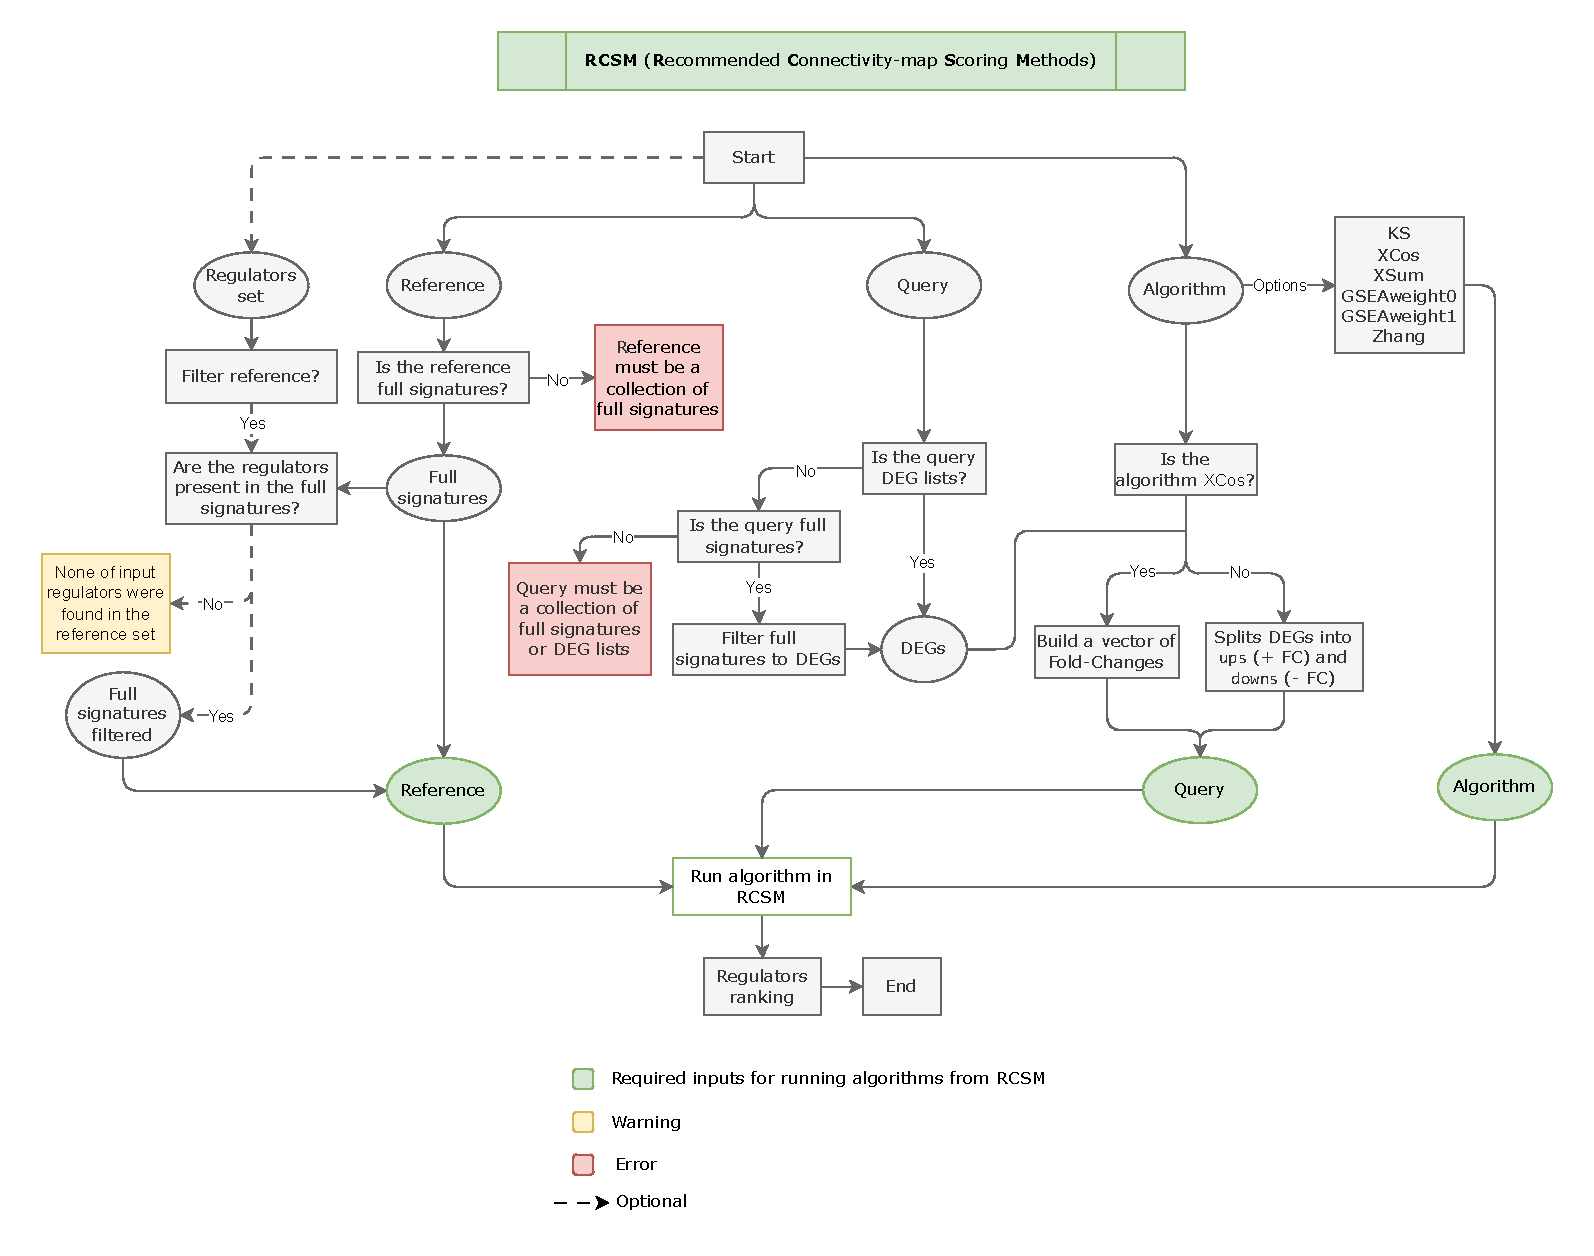
\includegraphics[height=4.5in]{fig3.2.RCSM}
    \caption[Flowchart representing the main steps for implementing connectivity mapping algorithms pre-built in the RCSM package.]{Flowchart representing the main steps for implementing connectivity mapping algorithms pre-built in the \gls{RCSM} package. The general computational pipeline for executing connectivity-based methods, showing the main input requirements, data preprocessing steps, algorithm execution, and output generation. Green indicates required inputs, while red highlights potential errors.}
    \label{fig:fig3.2.RCSM}
\end{figure}
%\end{newpdflayout}


\subsection{Pathway Enrichment} % (fold)
\label{sub:pathwayenrichment}

For running the enrichment-based algorithms, the decoupleR package~\cite{RN35} was used. 
The package was initially used to benchmark approaches for \gls{TF} activity inference. 
It contains 12 algorithms already implemented to expect prior knowledge resources (gene sets or regulons) to derive biological processes from omics data. 
Some of them take directionality into account (i.e., can work with regulon-gene set with activated and repressed genes). 
Of all the algorithms already implemented in decoupleR, only \gls{GSEA} and the others that respect directionality were considered for this benchmarking effort. As for \gls{CMap} algorithms, a shared wrapper function (Figure~\ref{fig:fig3.3.decoupleR}) was built to prepare the input and output data, designed to accept full signatures as query and regulon table or a gene regulatory network as reference data. If the reference is a list of signatures or \gls{DEGs}, it is converted to directed regulatory networks using the common filtering parameters described above. 
The implementation supports \gls{TF}-mode by filtering the network to keep only transcription-regulation edges. 
The query signatures are converted to a fold-change matrix and ID space conversions can also performed, if required to match network node identifiers. 
For algorithms that support directional information, the wrapper uses the edge type from the network.
% Extra parameters can be supplied to the argument list (Supplementary table 2).
The output of the wrapper function consists of regulator rankings with scores, effects, and p-values (if returned by the algorithm) organized by signature name and sorted by absolute score magnitude

\begin{figure}[htbp]
    \centering
    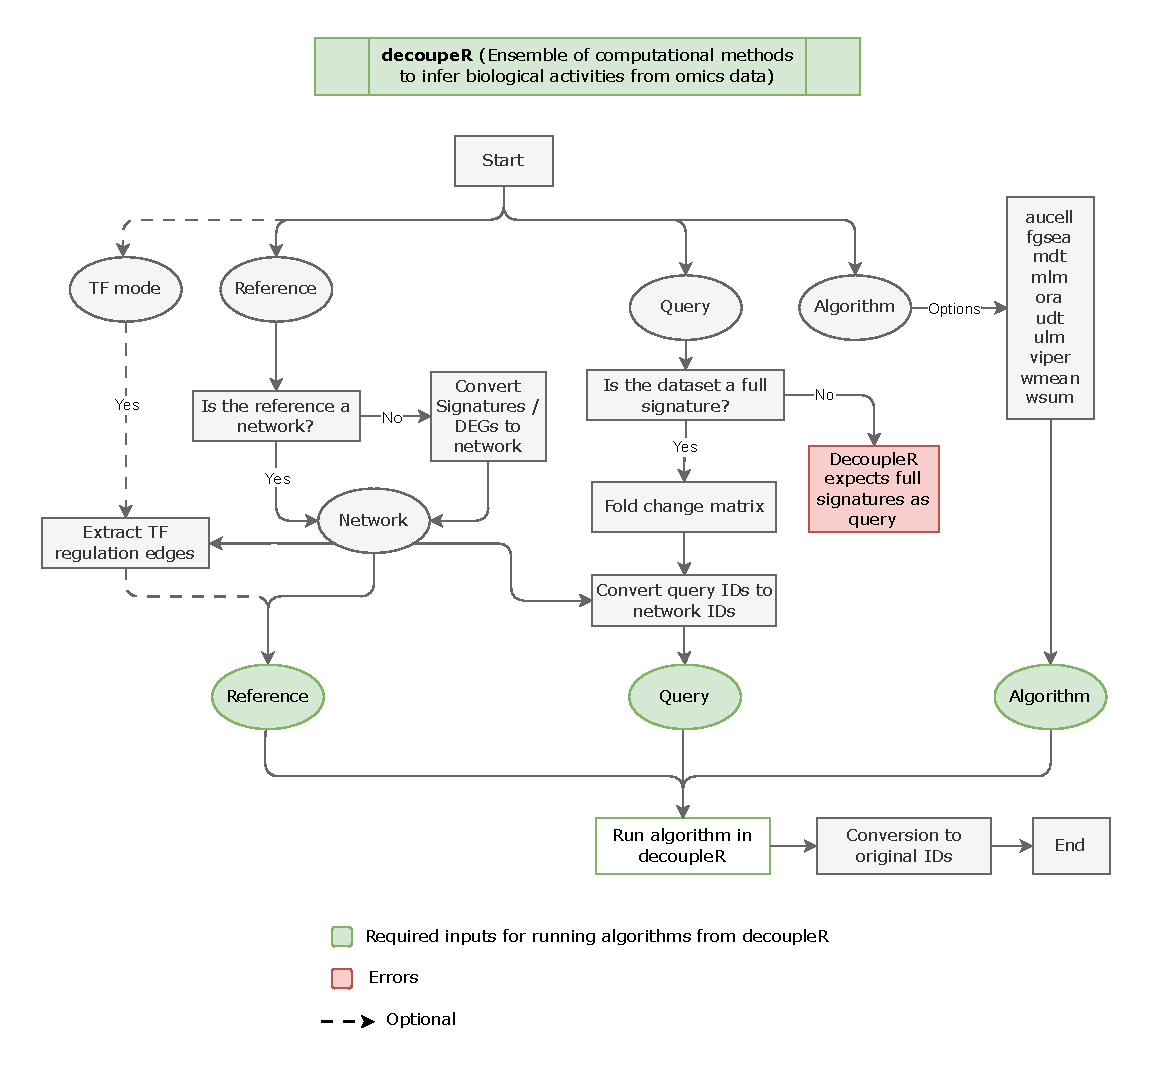
\includegraphics[height=5in]{fig3.3.decoupleR}
    \caption[Flowchart representing the main steps for implementing enrichment algorithms pre-built in the decoupleR package.]{Flowchart representing the main steps for implementing enrichment algorithms pre-built in the decoupleR package. The general computational pipeline for executing enrichment-based methods, showing the main input requirements, data preprocessing. Green indicates required inputs, while red highlights potential errors.}
    \label{fig:fig3.3.decoupleR}
\end{figure}
%\end{newpdflayout}


\subsection{Topology-based methods} % (fold)
\label{sub:topologybasedmethods}

\gls{CARNIVAL}~\cite{RN41} is prepared to integrate several types of prior knowledge (signed and directed \gls{PPI}, \gls{TF}-targets, and pathway signatures) to yield a causal subnetwork explaining the \gls{MoA} behind the observed omics data. This algorithm expects query \gls{DEGs} as input and a network as reference. \gls{CARNIVAL} wrapper (Figure~\ref{fig:fig3.4.CARNIVAL}) begins by validating essential inputs, including the CBC solver path required for the optimization engine.
It determines the execution mode based on whether perturbation targets and pathway weights are provided, enabling either the standard \gls{CARNIVAL} or the inverse \gls{CARNIVAL} algorithms. 
For reference network preparation, the wrapper handles multiple input formats by converting, if needed, signature collections or \gls{DEGs} lists into networks (with source node - interaction - target node).
The full signatures are also converted into matrix format. \gls{CARNIVAL} performs \gls{TF} activity inference with either a network-derived approach, if effect and mechanism are present, or using DoRothEA regulons from decoupleR. 
As an option, depending on the execution mode selected, a pathway activity score can be also calculated using PROGENy from decoupleR. 
The network is filtered to contain a subset of the interactions, keeping only nodes reachable from relevant \gls{TF}.
When \gls{CARNIVAL} algorithm is executed, the results are provided with regulator scores reflecting the frequency where each node appears in the causal subnetwork.

\begin{figure}[htbp]
    \centering
    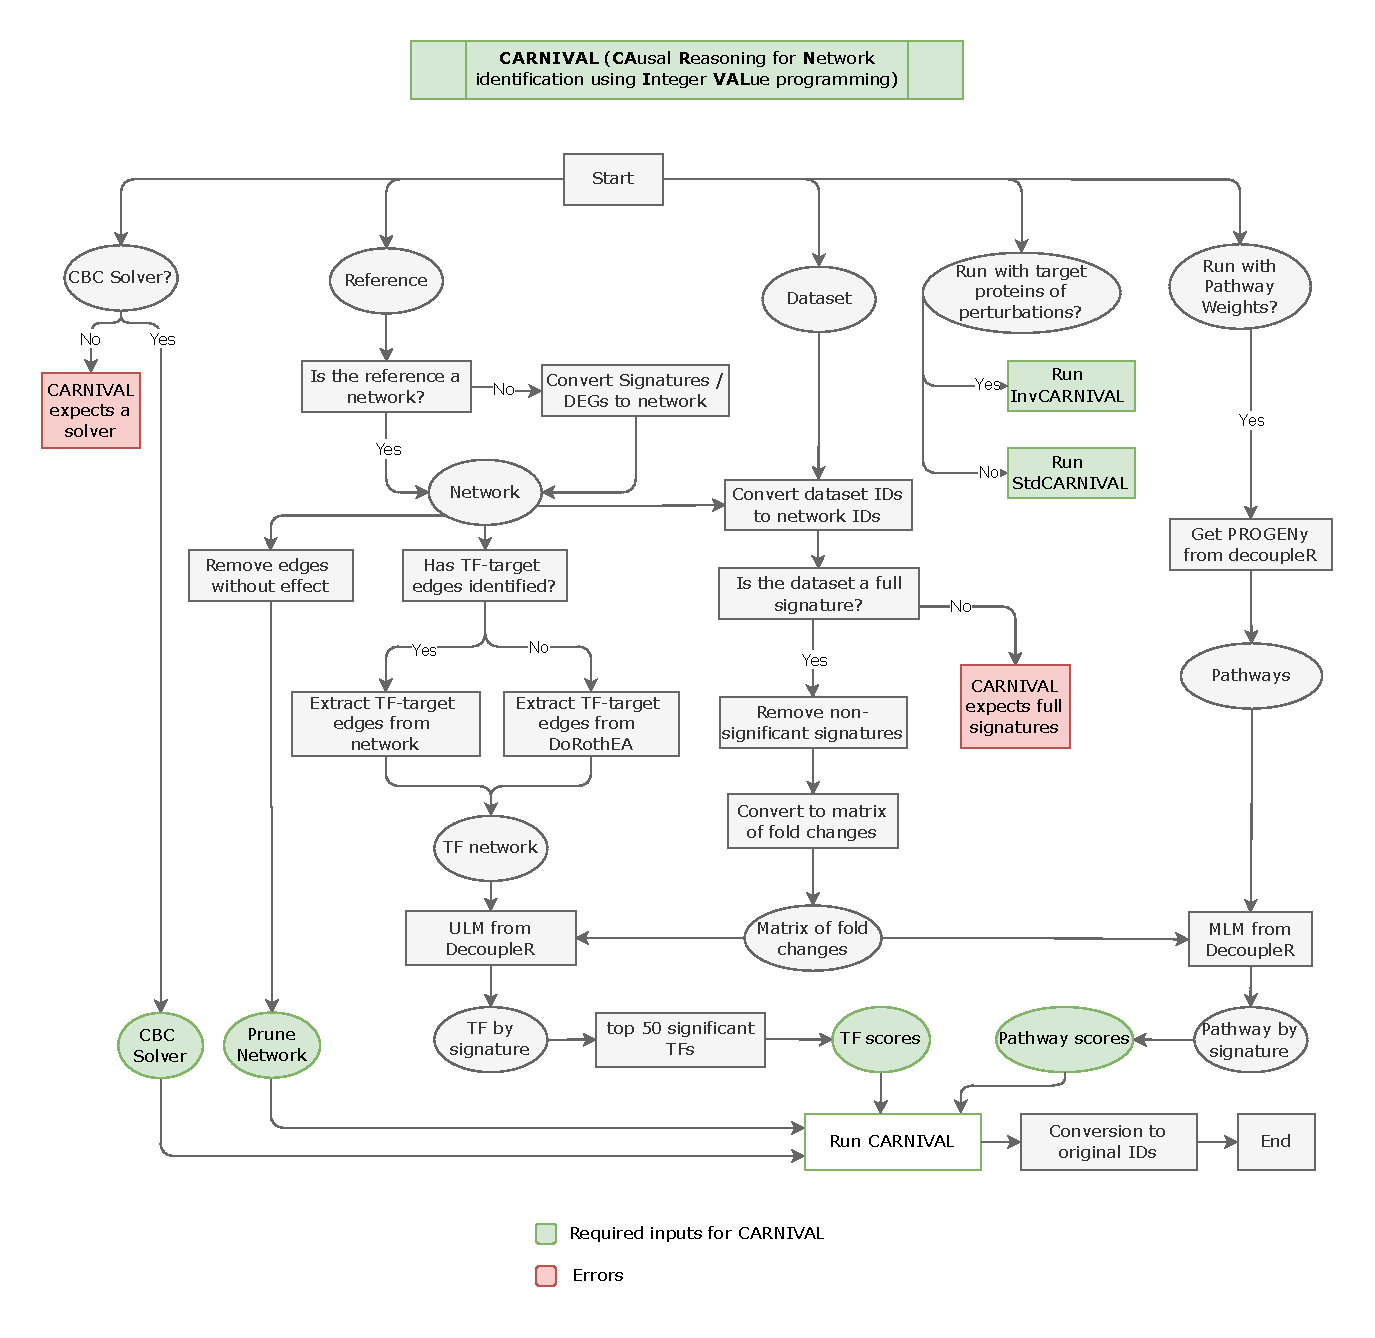
\includegraphics[height=5in]{fig3.4.CARNIVAL}
    \caption[Flowchart representing the main steps for implementing the CARNIVAL algorithm.]{Flowchart representing the main steps for implementing the \gls{CARNIVAL} algorithm. The general computational pipeline for executing this topology-based method, showing the main input requirements, data preprocessing steps, algorithm execution, and output generation. Green indicates required inputs, while red highlights potential errors.}
    \label{fig:fig3.4.CARNIVAL}
\end{figure}
%\end{newpdflayout}

\gls{ProTINA}~\cite{RN80} algorithm generates protein activity scores based on gene expression changes through network perturbation analysis.
The wrapper (Figure~\ref{fig:fig3.5.ProTINA}) starts by checking if the query is a collection of full signatures and if the reference data is a network.
If the reference is a signature or a \gls{DEGs} list, it is then converted to a network.
Then, query data is filtered to remove entire signatures without any \gls{DEGs}, as \gls{ProTINA} cannot process full profiles with only zero fold-change expression.
After that, the full signatures are converted to a matrix of fold changes, to remove genes that have zero standard deviation across all signatures. \gls{ProTINA} was originally designed to handle experiments with multiple replicates, time points, or dosages for each perturbation.
Since none of the data used for benchmarking have measurements in different conditions, the function only creates a vector with consecutive integers starting from one to the number of signatures, representing the number of groups.
Reference data is processed to construct a \gls{PGN}, which combines \gls{PPI} from the input network with \gls{TF}-target gene relationships.
From the \gls{PGN} it is calculated an adjacency matrix where rows represent proteins, columns represent genes, and matrix elements indicate the regulatory relationships.
Finally, the algorithm returns a matrix of protein (regulator) activity scores (signed Z-scores) for each perturbation group.
The wrapper converts the results back to gene symbols and ranks regulators by their activity scores, providing both magnitude and directionality of predicted protein activities.

\begin{figure}[htbp]
    \centering
    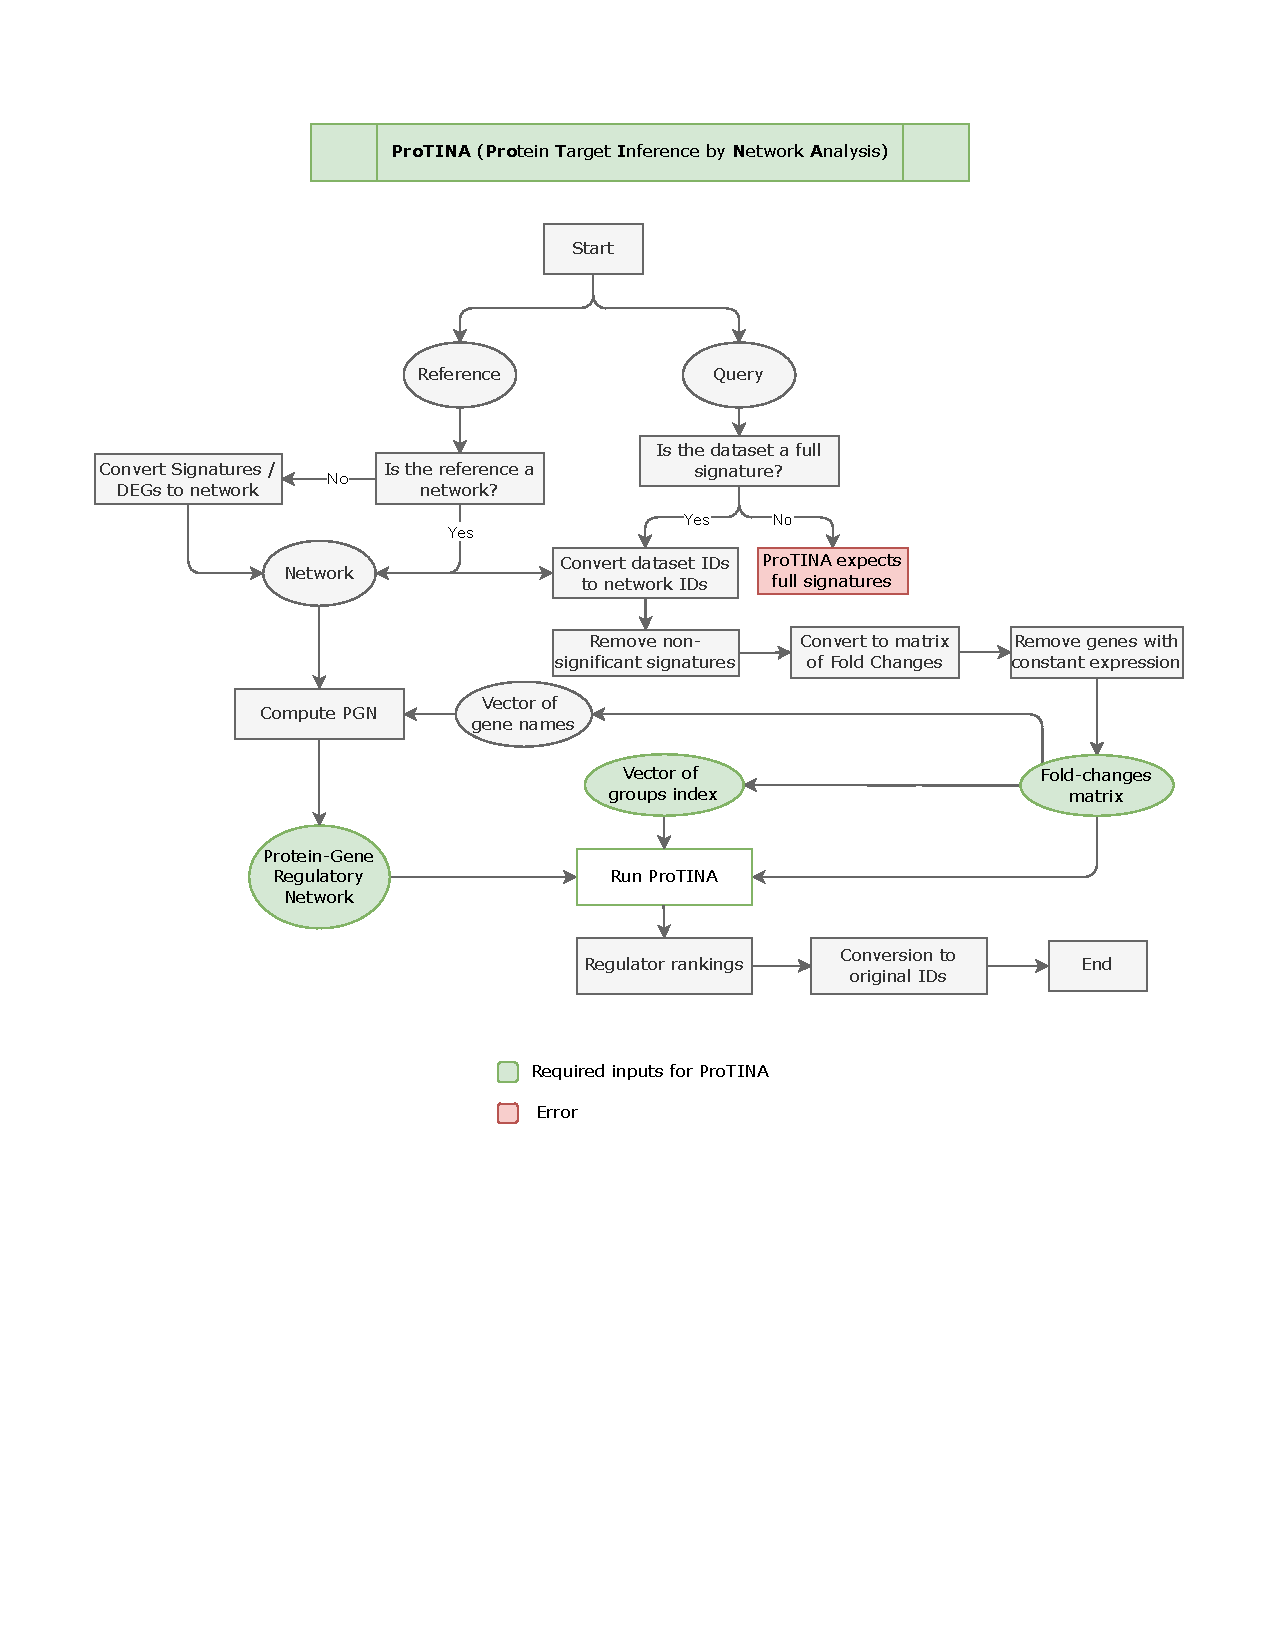
\includegraphics[height=5in]{fig3.5.ProTINA}
    \caption[Flowchart representing the main steps of ProTINA algorithm implementation.]{Flowchart representing the main steps of \gls{ProTINA} algorithm implementation. The general computational pipeline for executing this topology-based method, showing the main input requirements, data preprocessing steps, algorithm execution, and output generation. Green indicates required inputs, while red highlights potential errors.}
    \label{fig:fig3.5.ProTINA}
\end{figure}
%\end{newpdflayout}

To identify \gls{DEGs}, the CausalR~\cite{RN32} wrapper (Figure~\ref{fig:fig3.6.CausalR}) starts by processing the query signatures using the common filtering parameters described above.
The resulting data is then converted to the required CausalR format where genes are assigned with regulation status values (1 for upregulation, -1 for downregulation, 0 for unchanged).
Non-\gls{DEGs} within the signature are marked as unchanged, rather than excluded. The final format for the query dataset is a matrix with two columns for each experiment, reporting gene name and regulation status (1, -1, or 0) instead of fold-change values.
As for \gls{ProTINA}, signatures that do not have any \gls{DEGs} are removed. If reference data are not already provided in the correct format, the function can convert signature collections or \gls{DEGs} lists into directed causal networks.
Edges connect the regulators (signature names) to their targets (\gls{DEGs}) with edge effects corresponding to \gls{DEGs} fold-change signs. 
After having a network as reference, CausalR requires the construction of a \gls{CCG}, which contains twice the number of nodes and edges as each regulator is reported both as up and down/regulated.
CausalR allows two options of algorithms, RankTheHypotheses and runSCANR.
RankTheHypotheses algorithm uses the configurable path-length parameter delta, to control how many network edges can be traversed from regulator hypotheses to the observed gene expression data, enabling from a direct transcriptional regulation (delta = 1) analysis to a multi-step causal cascade (delta > 1).
Finally, the algorithm returns, per each signature, a regulator ranking with the regulator name, and the corresponding score (difference between correctly and incorrectly predicted \gls{DEGs}), p-value, and the predicted regulatory effect.

\begin{figure}[htbp]
    \centering
    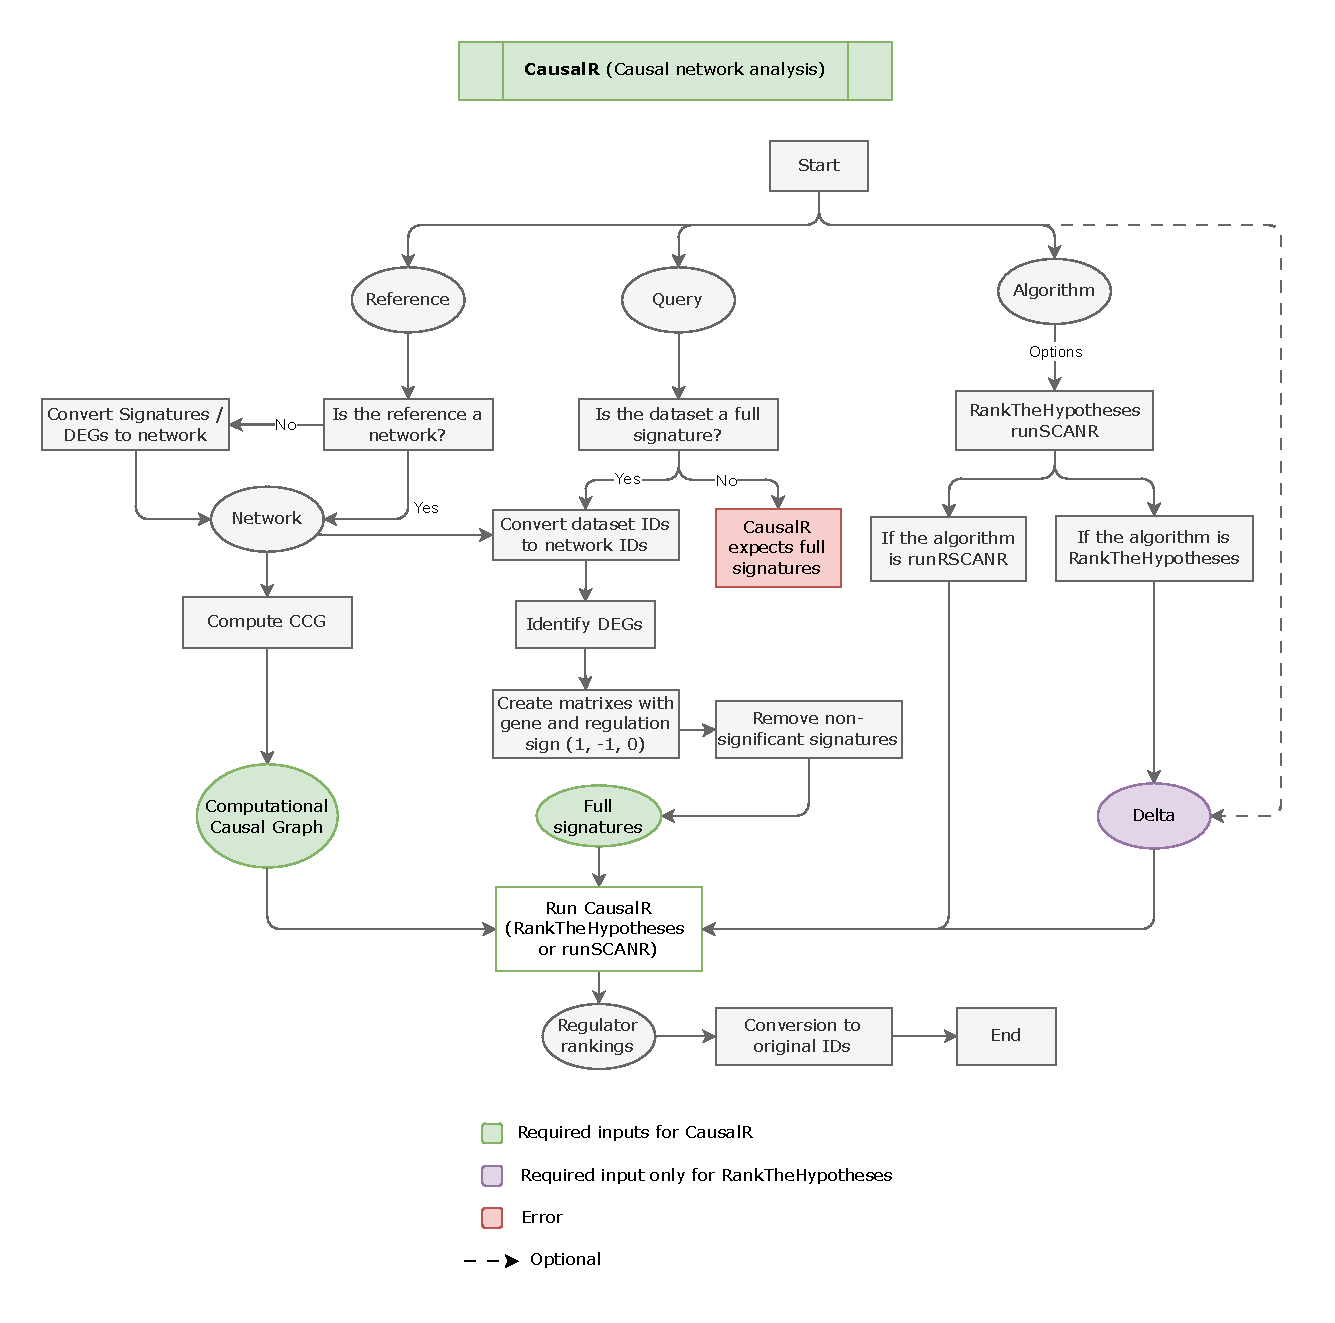
\includegraphics[height=5in]{fig3.6.CausalR}
    \caption[Flowchart representing the main steps of CausalR algorithm implementation.]{Flowchart representing the main steps of CausalR algorithm implementation. The general computational pipeline for executing this topology-based method, showing the main input requirements, data preprocessing steps, algorithm execution, and output generation. Green indicates required inputs, while red highlights potential errors.}
    \label{fig:fig3.6.CausalR}
\end{figure}
%\end{newpdflayout}

The \gls{CIE}~\cite{RN81} wrapper (Figure~\ref{fig:fig3.7.CIE}) starts by converting (if needed) full signatures to \gls{DEGs}, then transforming reference data into a network format.
A key aspect of this implementation involves preparing the network data structure to create two essential inputs: network entities (nodes) and network interactions (edges).
The entities data frame contains unique gene IDs classified as \gls{mRNA} or Protein based on the targets of the transcriptional regulation edges (mechanism = 1).
The relations data frame links source and target nodes using their distinct identifiers and maps the network edges with their regulatory effects.
The function supports three \gls{CIE} algorithms: Fisher for unsigned networks, Ternary for completely signed networks, and Quaternary for partially signed networks (default).
The results from \gls{CIE} are the regulators and the corresponding causal reasoning scores, regulatory effects, and a p-value ranking.

\begin{figure}[htbp]
    \centering
    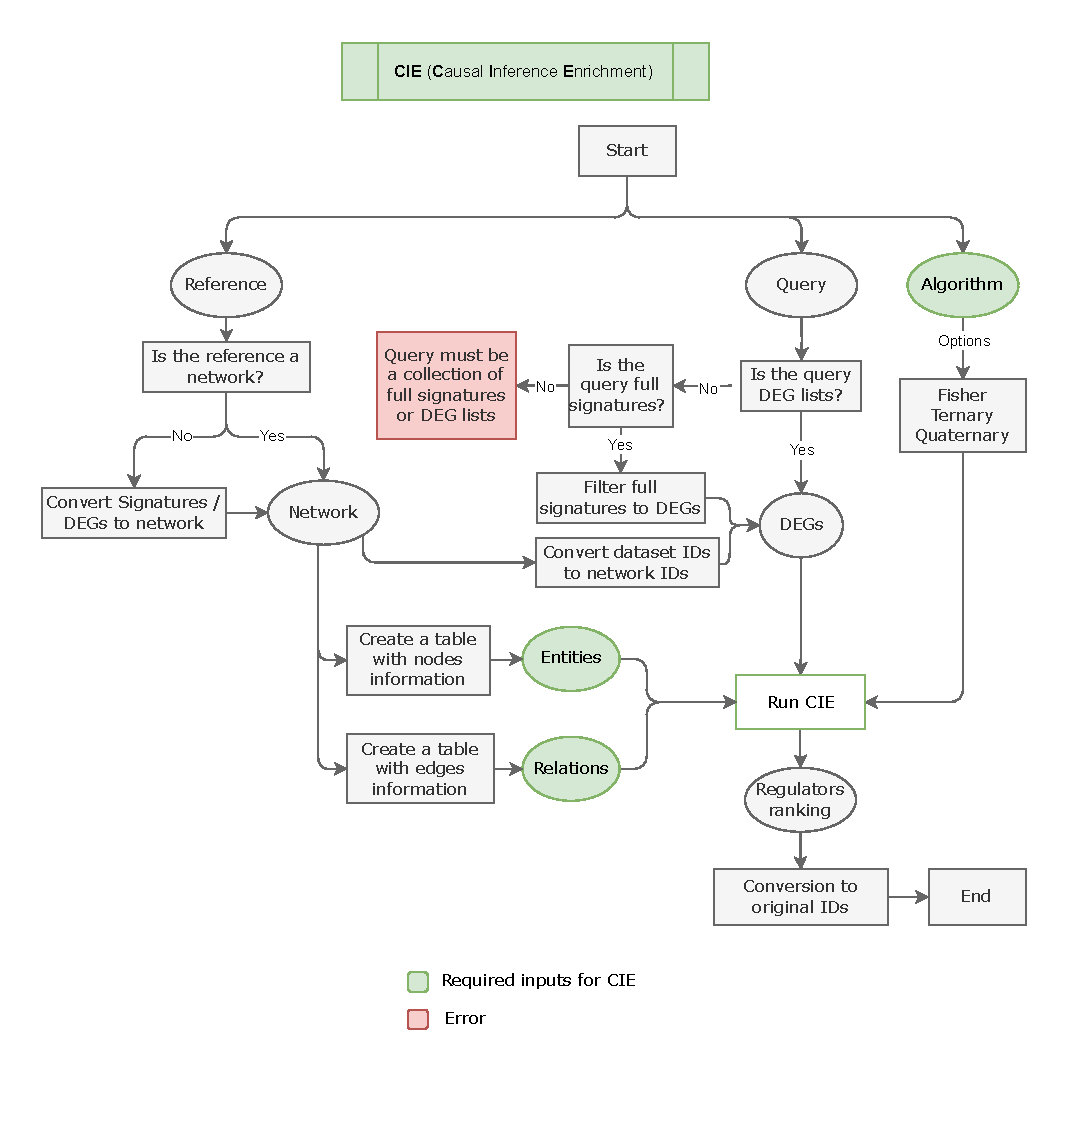
\includegraphics[height=5in]{fig3.7.CIE}
    \caption[Flowchart representing the main steps of CIE algorithm implementation.]{Flowchart representing the main steps of \gls{CIE} algorithm implementation. The general computational pipeline for executing this topology-based method, showing the main input requirements, data preprocessing steps, algorithm execution, and output generation. Green indicates required inputs, while red highlights potential errors.}
    \label{fig:fig3.7.CIE}
\end{figure}
%\end{newpdflayout}

As the other wrappers, athe one implemented for NicheNet~\cite{RN42} (Figure~\ref{fig:fig3.8.NicheNet}) also ensures that the input formats are correct by converting the input signatures to \gls{DEGs} and reference data to networks.
From the reference network, three subnetworks are created based on the regulatory mechanism: one ligand-receptor network and one signaling network from the signaling interactions (mechanism = 0), and one transcriptional network from gene regulatory interactions (mechanism = 1).
The ligand-receptor and signaling networks are constructed using an optional vector of regulators, which provides a list of source nodes to filter signaling interactions.
If this optional vector is not provided, only unique source nodes are used to create the set of regulators.
The ligand-receptor network includes only edges where the source node is a regulator, whereas the remaining edges are presented in the signaling network, with the downstream signaling cascades down to the target genes.
In the next step, a weighted network is constructed (\texttt{construct\_weighted\_networks}() function from nichenetr \gls{R} package~\cite{RN42}).
This function merges the three subnetworks into one graph, and assigns weights to edges based on their origin. By default, equal weights are assigned to all edge types (ligand-receptor, signaling, and gene regulatory).
To down-weight the influence of highly connected nodes, hub correction is applied to the network (\texttt{apply\_hub\_corrections}()).
With the weighted network, a ligand-target matrix is built (\texttt{construct\_ligand\_target\_matrix}()) containing target genes as rows, ligands as columns and scores for each entry (inferred signaling strength), from each ligand to each gene.
At this point, the inputs required to run NicheNet core function (\texttt{predict\_ligand\_activities}()) are ready: a vector of \gls{DEGs}, the full set of genes present in the ligand-target matrix (used as the background), the ligand-target matrix of regulatory scores and the list of ligands (regulators) to prioritize.
The output from NicheNet is ranked by corrected \gls{AUPR} scores and identifiers are converted back if needed.

\begin{figure}[htbp]
    \centering
    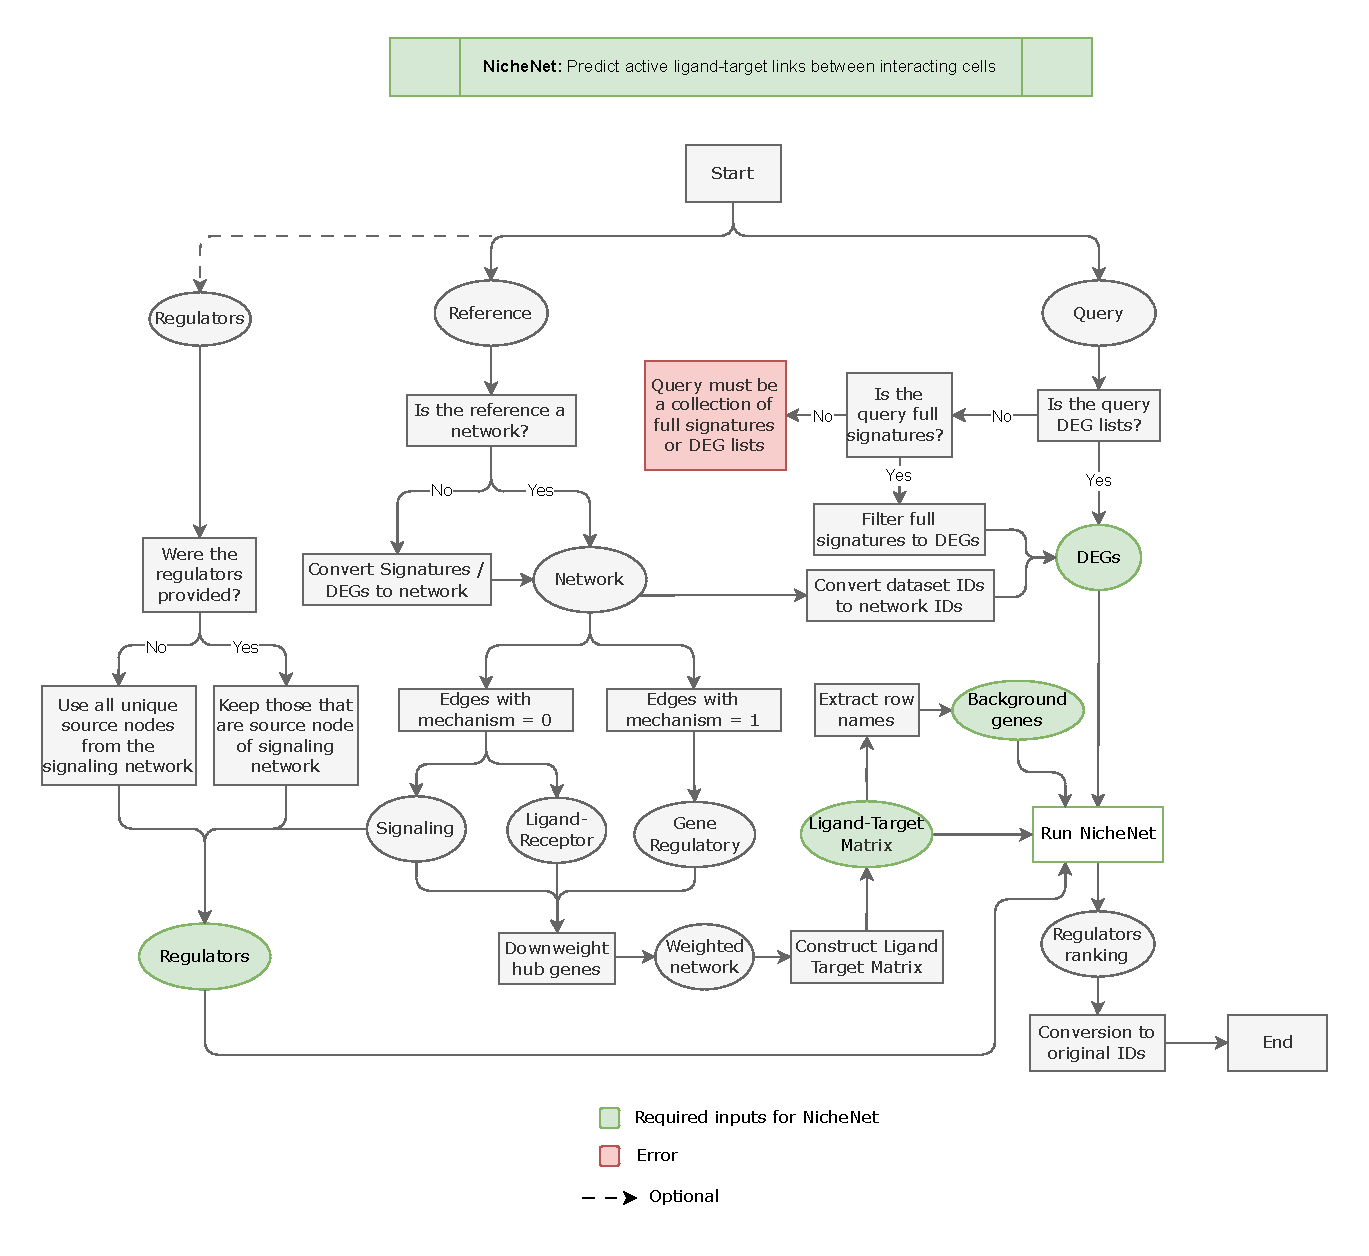
\includegraphics[height=5in]{fig3.8.NicheNet}
    \caption[Flowchart representing the main steps of NicheNet algorithm implementation.]{Flowchart representing the main steps of NicheNet algorithm implementation. The general computational pipeline for executing this topology-based method, showing the main input requirements, data preprocessing steps, algorithm execution, and output generation. Green indicates required inputs, while red highlights potential errors.}
    \label{fig:fig3.8.NicheNet}
\end{figure}
%\end{newpdflayout}

The implementation of the \gls{CBDD} wrapper functions (\gls{CBDD} baseline and \gls{CBDD} causal reasoning) follows an identical structure, with both functions sharing the same core preprocessing pipeline and output handling.
For this reason, they are both represented in a single schema, with the differences highlighted (Figure~\ref{fig:fig3.9.CBDD}).
Both start with validation and preprocessing of input data, converting query datasets to \gls{DEGs} lists, handling reference networks as described previously and performing ID conversion to map query genes/regulators to network-specific identifiers.
The wrapper functions then execute their respective algorithms, and return the results.
Despite the similarities, there are differences between the implementations that reflect their distinct computational requirements.
The \gls{CBDD} baseline function supports randomWalk, overconnectivity, interconnectivity, networkPropagation, and hiddenNodes algorithms, while \gls{CBDD} causal reasoning runs causalReasoning, SigNet, and quaternaryProd.
The causal reasoning wrapper requires network attributes such as the effect and mechanism, reflecting the need for directed, signed edges for causal inference.
Moreover, the \gls{CBDD} baseline converts networks to igraph objects, while \gls{CBDD} causal reasoning creates a causal graph.
Essentially, both wrappers return regulator scores, but since \gls{CBDD} causal reasoning considers directionality, the results contain additional information about the effect of the relationships (predicted activation or inhibition).

\begin{figure}[htbp]
    \centering
    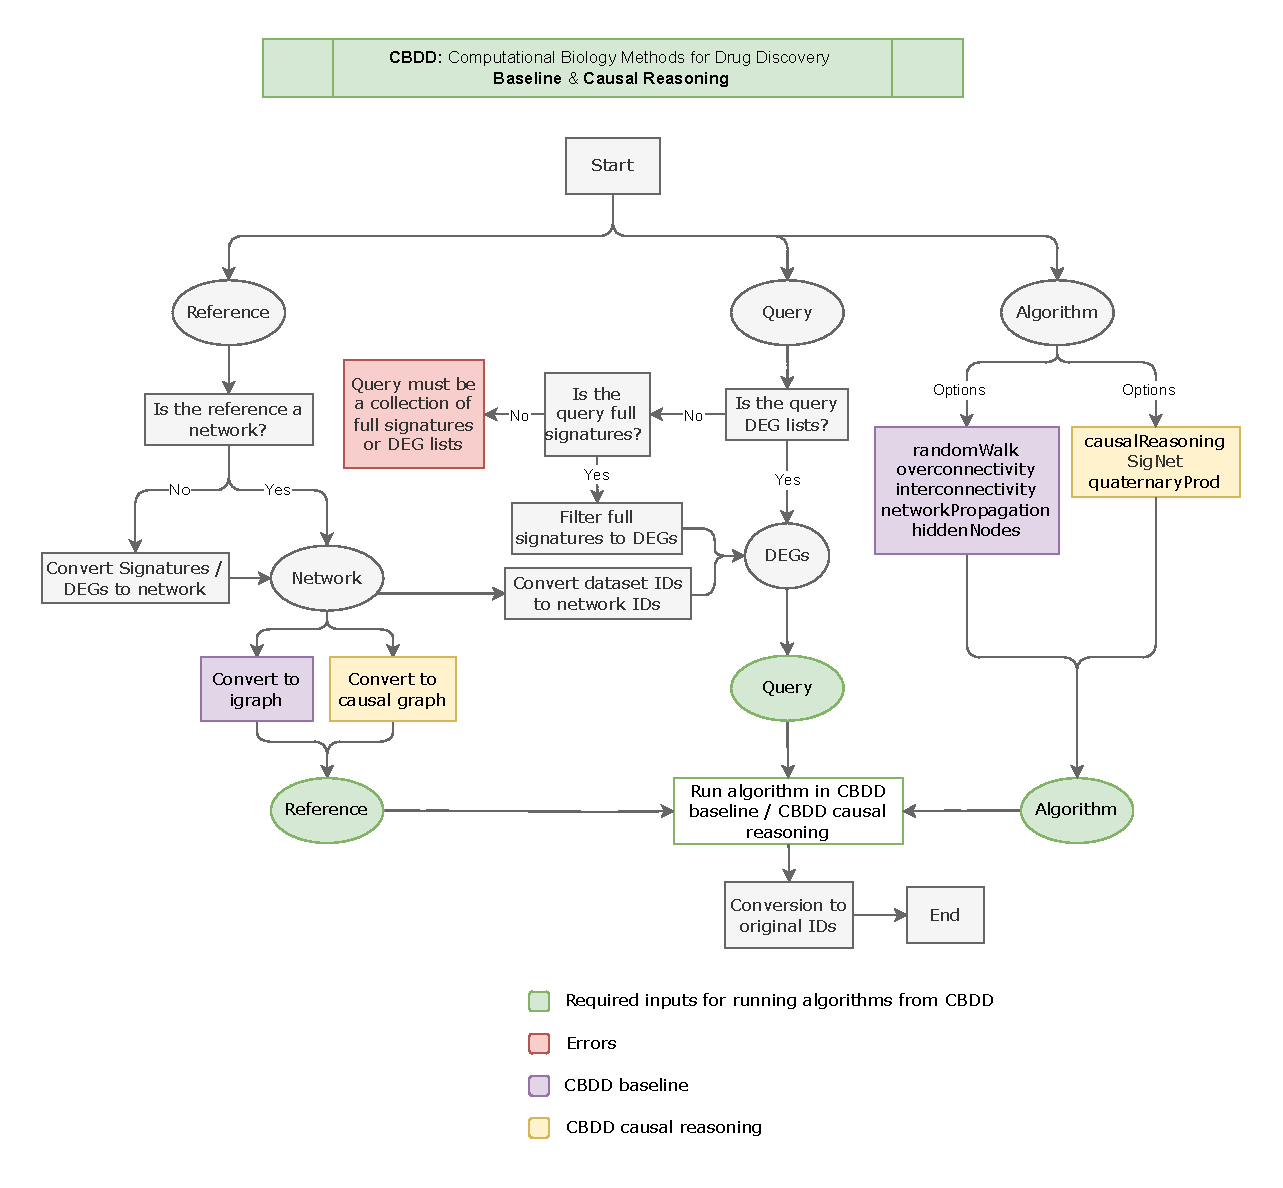
\includegraphics[height=5in]{fig3.9.CBDD}
    \caption[Flowchart representing the main steps of the wrapper function of both the CBDD baseline and CBDD causal reasoning algorithms implementation.]{Flowchart representing the main steps of the wrapper function of both the \gls{CBDD} baseline and \gls{CBDD} causal reasoning algorithms implementation. General computation pipeline and color coding as previously.}
    \label{fig:fig3.9.CBDD}
\end{figure}
%\end{newpdflayout}


\section{Evaluation} % (fold)
\label{sec:evaluation}

The final part of the study pipeline involves evaluating the algorithms by comparing the outputs from the algorithms' runs with the gold standard data.
This evaluation process involves three main steps: configuration, running the algorithm, and evaluating performance against the standards.
The configuration step includes selecting the input data (both the query and reference), as well as the standard with the verified list of the targets.
Then, the execution requires defining which algorithms to run for the selected input data.
Finally, the metrics are defined to assess performance of each algorithm, considering the known targets provided by the gold standard data. 

The evaluation was performed at the level of each signature, aggregating results to obtain an average assessment by dataset.
In general, the algorithms return all the ranked and scored regulators, so the threshold for considering which regulators are significant was also defined in two ways.
If an algorithm provides p-values for the regulators, the threshold of 0.05 is used to consider that regulator as significant (if p-value < 0.05).
If this is not the case, the top 1\% of regulators with the highest scores are selected.
In the case of \gls{CARNIVAL}, which returns a subnetwork, all the regulators in that network are already considered significant.

The performance was measured at a target and pathway level.
The former considers target recovery as the percentage of gold standard targets among all significant regulators, top 1\% and top 100 regulators.
Target enrichment was calculated using hypergeometric test enrichment ($-\log_{10}(\text{p-value})$), for the intersection of significant regulators and the gold standard targets.
It was also analyzed the rank of the top predicted gold standard target and target effect correctness, when directional information was available.
The target recall was measured at multiple percentage cutoffs (0.001\% to 1\% in 0.001\% steps) to enable the calculation of the \gls{AUPR}. This led to three general classifications:

\begin{enumerate}
\item Overall recovery: average of target recovery percentages, enrichment scores, and scaled \gls{AUPR} (for the top 1\%) across all signatures.

\item Recoverable signatures only: target recovery percentage calculated only on the subset of signatures whose true targets appear in the reference network.

\item	Win rate: to assess each algorithm's ability to identify actual target genes, the win rate represents how frequently a given output ranking contains a true target higher than all other competing algorithms. The \gls{WPAE} is obtained subtracting the expected win rate under random chance (1 divided by the number of algorithms), as the number of competing algorithms can change between runs. 
\end{enumerate}

The assessment of performance at the pathway level is equally important to understand whether the algorithm not only recovers the target itself, but also the biological pathways to which these targets are connected.
From the selected significant regulators, an enrichment analysis of the biological pathways was done using the \gls{CBDD} \texttt{enr} function, with MetaBase mapping gene sets to the pathways that are most associated with the targets predicted by the algorithms.
The statistical significance of the overlap between biological pathways identified from the targets and those manually annotated via MetaBase was calculated with a hypergeometric test (\texttt{hh\_pvalue}() function from \gls{CBDD}).
The result was recorded as a pathway enrichment score ($-\log_{10}(\text{p-value})$), where a higher score indicates that the algorithm is able to identify pathways directly affected by the perturbation. For comparing the results, the mean pathway enrichment score for each algorithm was computed by averaging those signatures whose true targets appear in at least one MetaBase pathway.

